\documentclass[a4paper,10pt,fleqn]{article}

\usepackage{src/common/layout}

\input{src/common/booleans}

\setboolean{STANDALONE}{true}

\newcommand{\EtPath}{src/BLDC}
\newcommand{\BIBLIOGRAPHY}{src/common/ET-Gruppe_Source}
\newcommand{\DasAndereTeam}{T27}
\newcommand{\BLDCTeams}{T27 und T32}
\newcommand{\BLDCcollab}{Dieses Kapitel ist eine Zusammenarbeit der Gruppen \BLDCTeams. }

\begin{document}
	\begin{titlepage}

\begin{center}

% Oberer Teil der Titelseite:
%\includegraphics[width=0.15\textwidth]{./logo}\\[1cm]    
\textsc{\LARGE Produktentwicklung 2}\\[1.5cm]

\textsc{\Large Hochschule Luzern\\
    ~\\
    Technik \& Architektur}\\[0.5cm]

\vfill{}

% Title
\newcommand{\HRule}{\rule{\linewidth}{0.5mm}}
\HRule \\[0.4cm]
{   \Huge \bfseries Review ET-Gruppe\\
        ~\\
        \large Rückblick auf die ET-Zusammenarbeit}\\[0.4cm]

\HRule \\[1.5cm]

% Author and supervisor
\begin{minipage}[t]{0.4\textwidth}
    \begin{flushleft} \large
        \emph{Autoren:}\\
        Ervin \textsc{Mazlagi\'c}\\
        Flavio \textsc{Kreiliger}\\
        Bettina \textsc{Wyss}\\
        Daniel \textsc{Winz}\\
        Yves \textsc{Studer}\\
    \end{flushleft}
\end{minipage}
\hfill
\begin{minipage}[t]{0.4\textwidth}
    \begin{flushright} \large
        \emph{Projektgruppe:} \\
        PREN-ET
    \end{flushright}
\end{minipage}

\vfill{}
\vfill{}
\vfill{}

% Unterer Teil der Seite
{\large Horw\\ \today}

\end{center}

\end{titlepage}

	\tableofcontents
	\newpage
	\input{src/common/Hardwarezusammenarbeit}
	\input{src/BLDC/Ansteuerung}
	\newpage
	\ifSTANDALONE
\section{Prinziptest}
\fi
\ifEMBED
\subsubsection{Aufbaubeschreibung}
    \BLDCcollab \\
\fi
\ifEMBED
    \begin{wrapfigure}{r}{0.55\textwidth}
       	\includegraphics[scale=0.4]{\EtPath/Bilder/MotoransteuerungSchema.jpg}
       	\centering
       	\caption{Schema des Brushless-Versuchsaufbaus}
        \label{abb:MotoransteuerungSchema}
    \end{wrapfigure}
\fi
    Das Schema des Gesamtaufbaus des Tests ist in der Abbildung 
    \ref{abb:MotoransteuerungSchema} ersichtlich. Die 3-Phasen H-Brücke im 
    oberen grünen Rechteck wird direkt vom FPGA 
    \footnote{\textbf{F}ield-\textbf{P}rogrammable \textbf{G}ate 
    \textbf{A}rray} angesteuert. Die Hardware dieser Brücke ermöglicht eine 
    voll galvanisch getrennte Ansteuerung mit $3.3 V$ Logikpegeln. Diese 
    Brücke wurde zur Verfügung gestellt und direkt verwendet. Die 
    Rekonstruktion der Hallsensoren-Signale findet im rot markierten Teil des 
    Aufbaus statt. Dieser Part wird auf einer Laborplatte aufgebaut und 
    gelötet. Die so generierten Signale $U_{Hallsensor}$, $V_{Hallsensor}$, 
    $W_{Hallsensor}$ werden einem FPGA geliefert. Anhand dieser Signale 
    steuert das FPGA die H-Brücken-Transistoren mit den Signalen $U_h$, $U_l$, 
    $V_h$, $V_l$, $W_h$, $W_l$. Die im FPGA enthaltene Konfiguration besteht 
    aus simplen AND-Verknüpfungen, die die anliegenden Signale sehr schnell 
    und effizient verarbeiten können. Auf diese Weise ist es möglich, den 
    Motor sehr schnell anzusteuern.
    \ifSTANDALONE
    \begin{figure}[h!]
    	\includegraphics[scale=0.4]{\EtPath/Bilder/MotoransteuerungSchema.jpg}
       	\centering
       	\caption{Schema des Brushless-Versuchsaufbaus}
        \label{abb:MotoransteuerungSchema}
    \end{figure}
    \fi
    In der Abbildung \ref{abb:MessplatzAufbau} ist der gesamte Aufbau 
    abgebildet. Man beachte die markierten Felder. Am linken unteren Rand ist 
    der Motor befestigt. In der Mitte des Bildes ist die Hardware zur 
    Rekonstruktion der Hallsensoren-Signale.  Die generierten Signale werden 
    dem FPGA in der unteren linken Ecke zugeführt. Diese Signale werden 
    logisch verknüpft und danach die sechs Signale generiert, um die H-Brücke 
    in der rechten oberen Hälfte anzusteuern.  Die H-Brücken wiederum treiben 
    den Motor an.
    \begin{figure}[h!]
    %\vspace{-16pt}
       	\includegraphics[width=0.9\textwidth]{\EtPath/Bilder/MessplatzAufbau.jpg}
       	\centering
       	\caption{Testaufbau} 
        \label{abb:MessplatzAufbau}
    %\vspace{-10pt}
    \end{figure}
    Die im FPGA enthaltene Logik basiert auf der Wahrheitstabelle, die in 
    Tabelle \ref{abb:WahrheitstabelleAnsteuerung} abgebildet ist.

\ifSTANDALONE
\subsection{Messmittel}
\fi
\ifEMBED
\newpage
\subsubsection{Messmittel}
\fi
    \begin{table}[h!]
        \centering
        \begin{zebratabular}{lll}
            \rowcolor{gray}
            Gerät &
                Typ &
                Nummer \\
            Speisegerät & 
                Rohde \& Schwarz NGSM 32/10 &
                Inv.-Nr. 009 \\
            Oszilloskop &
                Agilent MSO6052A &
                Inv.-Nr. 44; S/N: MY44001903 \\
            Mainframe &
                Hameg HM8001-2 &
                SN: 059520046 \\
            Speisegerät &
                Hameg HM8040-3 &
                SN: 015405014 \\
            Pulsgenerator &
                Hameg HM8035 &
                Inv.-Nr. 44 \\
        \end{zebratabular}
        \caption{Messmittel des Versuchsaufbaus}
    \end{table}

\ifSTANDALONE
\subsection{Resultat}
\label{chap:VersuchsResultat}
\fi
\ifEMBED
\subsubsection{Resultat}
\label{chap:VersuchsResultat}
\fi
Mit dem beschriebenen Aufbau konnte ein BLDC-Motor erfolgreich angesteuert 
werden. Wie in Abbildung \ref{abb:MessplatzAufbau} am linken unteren Rand zu 
erkennen ist, ist an der Motorwelle eine Aluminiumplatte montiert. Mit dieser 
und eines Magneten konnte der Motor mittels einer Wirbelstrombremse belastet 
werden. Auf diese weise konnte rund $120 W$ elektrische Leistung umgesetzt 
werden. Dabei stellte sich heraus, dass die PWM nachgeregelt werden muss, wenn 
eine Last getrieben wird. Weiter bietet der Aufbau, wie er getestet wurde 
keine Möglichkeit den Motor ohne äussere Manipulation zu starten.\\
\\
Diese beiden Tatsachen sprechen dafür, dass das Prinzip grundsätzlich 
funktioniert. Für die Realisierung würde sich ein eigenes Board anbieten, auf 
dem ein eigener Controller die Regelung und die Zwangskommutierung beim 
Starten des Motors übernimmt.

	\newpage
	\ifSTANDALONE
\section{Fallback}
\fi
\ifEMBED
\subsubsection{Fallback}
\fi
Ist der Einsatz des vorgesehenen BLDC-Treibers nicht möglich, so muss eine
alternative Ansteuerung erfolgen. Eine solche kann mit einer handelsüblichen
Steuerungen aus dem Modellbau erfolgen. Eine solche BLDC-Steuerung ist per
PWM angesteuert, wobei die im Modellbau üblichen Signale gelten, wie in der
Abbildung \ref{fig:rc-pwm} dargestellt.

\begin{figure}[h!]
	\centering
	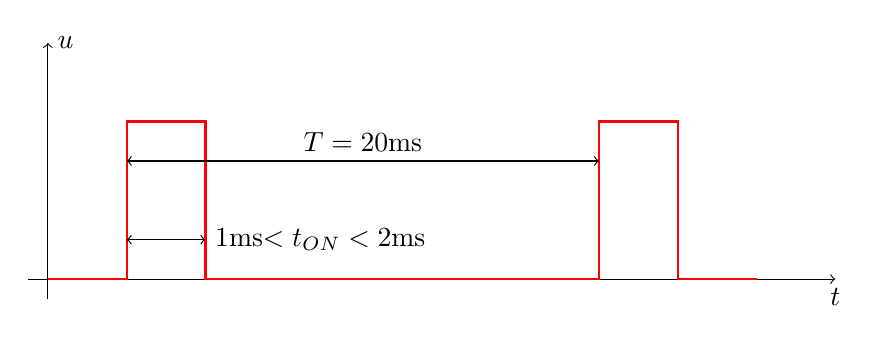
\begin{tikzpicture}
		% Achsen
		\draw[->] (-0.25,0) -- (10,0) node[anchor=north] {$t$};
		\draw[->] (0,-0.25) -- (0,3) node[anchor=west] {$u$};
		% Signal
		\draw[-,red,thick] (0,0) -- (1,0) -- (1,2) -- (2,2) -- 
			(2,0) -- (7,0) -- (7,2) -- (8,2) -- (8,0) -- (9,0);
		% Zeiten
		\draw[<->] (1,1.5) -- (7,1.5) node[midway, above] {$T=20$ms};
		\draw[<->] (1,0.5) -- (2,0.5) node[right] {$1$ms$<t_{ON}<2$ms};
	\end{tikzpicture}
	\caption{Signalverlauf eines typischen Modellbau-PWM Signals}
	\label{fig:rc-pwm}
\end{figure}

Der Einsatz von Modellbausteuerungen für BLDC-Motoren erfordert ein
Feedback der Drehzahl, da diese lediglich eine Steuerung darstellen. Die
Drehzahlregelung muss über eine externe Einheit erfolgen, beispielsweise einen
Mikrocontroller. Solche BLDC-Steuerungen werden im Modellbau typischerweise als
\emph{Regler} vertrieben und sind auch für hohe Leistungen durchaus preiswert.

\ifSTANDALONE
\subsection{Konzeptbeschreibung}
\fi
\ifEMBED
\newpage
\paragraph{Konzeptbeschreibung}$~~$\vspace{2mm}\\
\fi
Um eine Regelung der Drehzahl des BLDC-Motors zu ermöglichen, bedarf es eines
Feebacks, welches die Drehzahl wiedergibt. Dies ist mit einem
Hall-Effekt-Schalter zu realisieren. Dieser reagiert auf die Magnetfelder,
welche durch Magnete auf dem Rotationskörper gegeben sind. Aus solch einem
Aufbau resultiert ein Feedback, welches mit Impulsen einen Segmentdurchlauf
des Rotationskörpers wiedergibt, wie in Abbildung \ref{fig:fallback-sketch}
dargestellt.
\begin{figure}[h!]
	\centering
	\includegraphics[width=0.8\textwidth]{\EtPath/Bilder/fallback_sketch_1.pdf}
	\caption{Erste Skizze des Fallback-Konzepts}
	\label{fig:fallback-sketch}
\end{figure}
Dieses Feedback wird mittels eines Mikrocontrollers ausgewertet und regelt
damit den Input der Steuerung mit dem PWM-Signal beziehungsweise der Impulsdauer.
Das Einlesen einer Flanke, die Zeitmessung bis zur nächsten Flanke und die
Stellung eines PWM-Signals, sind Tasks welche übliche Mikrocontroller direkt
durch ihre Peripherie-Module ausführen können. Dies ermöglicht eine einfache
Adaption in ein bestehendes Modell, denn es werden lediglich zwei Timer-IO
für diesen Fallback verwendet. Je nach Mikrocontroller ist ein Pegelwandler
für die PWM-Signale notwendig.

	\newpage
	\input{src/BLDC/encoder}
	\clearpage
	\setlength\bibitemsep{1.5\itemsep}
%Folgende Zeile auskommentieren, damit nur gebrauchte Literatur erscheint
\nocite{*}
\renewcommand{\refname}{Literatur- und Quellenverzeichnis}
% \bibliographystyle{apacite} set in layout.sty -> do not try to set it here again!
\bibliography{\BIBLIOGRAPHY}

	\listoffigures
	\listoftables
\end{document}
